%%%%%%%%%%%%%%%%%%%%%%% file typeinst.tex %%%%%%%%%%%%%%%%%%%%%%%%%
%
% This is the LaTeX source for the instructions to authors using
% the LaTeX document class 'llncs.cls' for contributions to
% the Lecture Notes in Computer Sciences series.
% http://www.springer.com/lncs       Springer Heidelberg 2006/05/04
%
% It may be used as a template for your own input - copy it
% to a new file with a new name and use it as the basis
% for your article.
%
% NB: the document class 'llncs' has its own and detailed documentation, see
% ftp://ftp.springer.de/data/pubftp/pub/tex/latex/llncs/latex2e/llncsdoc.pdf
%
%%%%%%%%%%%%%%%%%%%%%%%%%%%%%%%%%%%%%%%%%%%%%%%%%%%%%%%%%%%%%%%%%%%


\documentclass[runningheads,a4paper]{llncs}

\usepackage{amssymb}
\setcounter{tocdepth}{3}
\usepackage{graphicx}
%%%%%%%%%%%%%%% New package
\usepackage{amsmath}
\usepackage{caption}
\usepackage{subfig}
\usepackage{csvsimple}
\usepackage{multirow}
\usepackage{array}
\usepackage{booktabs}
%%%%%%%%%%%%%%%
\usepackage{url}
\usepackage{float}
% \urldef{\mailsa}\path|{soltanin, locheng, ingrid.haas, frank.holzwarth,|
% \urldef{\mailsb}\path|anna.kramer, leonie.kunz, christine.reiss, nicole.sator,|
% \urldef{\mailsc}\path|erika.siebert-cole, peter.strasser, lncs}@springer.com|
% \newcommand{\keywords}\cite{1}{\par\addvspace\baselineskip
% \noindent\keywordname\enspace\ignorespaces#1}

\begin{document}

%\mainmatter  % start of an individual contribution

% first the title is needed
\title{Audio-visual speech enhancement and background noise removal}

% a short form should be given in case it is too long for the running head
%\titlerunning{Lecture Notes in Computer Science: Authors' Instructions}


% the name(s) of the author(s) follow(s) next
%
% NB: Chinese authors should write their first names(s) in front of
% their surnames. This ensures that the names appear correctly in
% the running heads and the author index.
%
\author{Han Geng\and Chen Li}
%\thanks{Please note that the LNCS Editorial assumes that all authors have used
%the western naming convention, with given names preceding surnames. This determines
%the structure of the names in the running heads and the author index.}%

%%
%\authorrunning{Lecture Notes in Computer Science: Authors' Instructions}
% (feature abused for this document to repeat the title also on left hand pages)

% the affiliations are given next; don't give your e-mail address
% unless you accept that it will be published
\institute{Group Name: Mariana}

%
% NB: a more complex sample for affiliations and the mapping to the
% corresponding authors can be found in the file "llncs.dem"
% (search for the string "\mainmatter" where a contribution starts).
% "llncs.dem" accompanies the document class "llncs.cls".
%

% \toctitle{Lecture Notes in Computer Science}
% \tocauthor{Authors' Instructions}
\maketitle


\begin{abstract}

Audio-visual speech enhancement is a coding process that suprsses the unwanted noise to highlight the useful audio signal from complex audio and video input. Recent development on video processing and audio quality enhancement provides better visual and aural experience, with the involve of deep neural network, audio/video enhancement will be improved compared to traditional method. The goal of this project is to implement a deep audio-visual speech enhancement network, which will be used to remove background noise from a given speaker video with its corresponding audio spectrogram. For research convenience, the video frames will be focused on the lip region only, and the corresponding audio clips used for both training and experiment will be a mix of the original noise-free audio signal and some generated noise signal. The program will initialize with data provided by a pre-trained network on a word-level lip-reading task, who contains labeled speaker videos and their corresponding noiseless audio signals. Our speech enhancement network will take in as input these data, where noise will be added into the audio signals, complete the training process, and then give the audio spectrum with noise removed as output. This method is different from the automatic speech recognition (ASR) who can only identify speech in a relatively noiseless environment. Instead, it can be applied to a more noisy environment where the magnitude of noise is much higher than usual (low signal-to-noise ratio), and it will also work in multi-speaker environments (such as News conference with translater's voice)
\end{abstract}


\section{Introduction}
Recent development on video processing and audio quality enhancement gives us better visual and aural experience, and the application of machine learning makes it possible for voice recognition which makes our lives even more convenient. But in the process of training and testing, the input voice signal must be recorded under relatively noiseless environment, otherwise the noise signal in the sound spectrum will cause serious deterioration in the performance, for the reason that the noise signal would add unwanted fluctuation in the spectrum and cause the spectrum to have different characteristics from its original shape, hence the machine would not recognize it as what it should be.\\
 
The major themes and applications of Automatic Speech Recognition was discussed in this paper \cite{1} in 2010, and it proposes several approaches and challenges faced by researchers in this field. For example, the context of the speech, the environment quality of the speech and the speakers themselves would influence how well the task could perform. The models proposed supports several types of speech recognition, such as isolated words, connected words, continuous speech and spontaneous speech. In order to recognize these forms of words and speech, a quiet environment must be ensured because for isolated words especially, the recognizers must obtain a test sample that does not have noise or audio signal on either side of the sample window. Imagine using Siri in a crowded station or in strong wind, it may not be able to receive exact orders that you give under such noisy environment. Maybe Siri is not a good example, but it does represent such a situation where the speech recognition system may not function as we want it to be, because of the presence of noises. Other related applications that involve outdoor or noisy activities can also be affected by low signal-to-noise ratio, such as gambling, helicopters and battleground intelligent management systems, etc.\\
 
Because of the development of speech recognition and other technical advances, people are having higher and higher demand on audio signal quality, which is often contaminated by numerous sources of natural and artificial noises. In order to improve audio quality and increase voice signal clearness, the development of voice signal enhancement and noise removal is essential.\\
 
Various graphic enhancement and noise removal techniques make it easier for us to extract useful information by recovering video or audio clips damaged by multiple source of noise, and the clearer audio signal can then be used in speech recognition and other field of applications.\\

Multiple advanced approaches to voice enhancement and noise removal have been proposed over the past few years, the most direct approach is using only audio to segregate monaural speech as supposed in \cite{2} in 2009, which is a little bit different from what we are going to propose (remove noise from single-speaker speech), but the core concept is rather similar. \cite{2} uses supervised learning techniques and computational auditory scene analysis to segregate speech recorded in one-microphone scenario. It focused mainly on the noises caused by room reverberation, which cause severe degradation to voice signal quality and is rather hard to resolve because the reverberating noise signal are mainly repetition of ground truth signal but in lower volume, hence it has similar patterns in audio spectrum as ground truth. This makes it hard for researchers to isolate just one channel of clear voice signal, and even harder when there are multiple speakers in the room, each making speeches and causing room reverberation simultaneously. Since the research only uses audio signal, the major resolution technique is to use inverse filtering, but as the paper suggested, this approach is sensitive to room condition, and the result varies for different indoor settings and reverberation conditions. They proposed a method using supervised learning approach to set up several groups for a period of time-frequency (T-F) unit, each contains a set of harmonic characteristics, then they estimate a binary mask for the time-frequency unit, and this mask filters through all the local T-F units and removes those reverberant mixtures whose target energy is weaker than the interference energy. Value 1 in the mask represents that the target is stronger than the interference, and value 0 represents the opposite.\\

\begin{figure}[h!]
%\centering
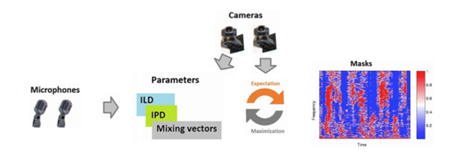
\includegraphics[scale=0.58]{fig1.png}
\caption{The direct path parameter vector is calculated with the help of video cameras. 
(The final probabilistic mask formed from the resulting probabilistic model is used for source separation)}
\label{fig:framework}
\end{figure}

As human beings when we are listening to multiple simultaneous speeches or single-speaker speech with strong noise, we are still able to distinguish the target speaker that we want to hear from other unwanted interfering noises. One reason being that we are using two ears for audio input which gives more characterizing information about the target speaker, but the most helpful and obvious devices that we use to distinguish target speaker is through our eyes.\\
 
Since we can observe visual information about our surroundings, we know when the speaker is talking when we see their mouths moving, and from this we know precisely which part of audio clips contains the speech that we desire, and everything happening outside the range of mouth movement is considered noises automatically. With the help of the video information, we can even generate audio signals from a silent video clip if we have trained a model to identify mouth movement and match it to words and sentences as discussed in \cite{3}, but this is beyond the scope of the topic of interest. Nevertheless, we can reduce the workload by a great amount and focus on removing noises from only part of the whole audio samples that contains the target speaker’s speech, if we have the visual information about the speaker and align it chronologically with the audio samples. The use of corresponding video signals as reference for speaker separation is proposed in \cite{4}. This paper focused on separating single-channeled speakers with help of corresponding visual information.\\
 
They record simultaneous speeches given by multiple speakers through a single-channel microphone, and capture videos of these speakers when they are giving the speeches. Using similar techniques as described above, they create a T-F binary mask generated from the visual information that defines which part of the audio is corresponding to the speaker video clip, then filter through the audio signals to retain the dominant speech signals. In this binary mask, value of 1 means the target speaker is talking, and 0 means the speaker is not talking and thus T-F unit is masked. The point of this method is to estimate which part of the T-F component and frequency unit should be retained.\\

\begin{figure}[h!]
%\centering
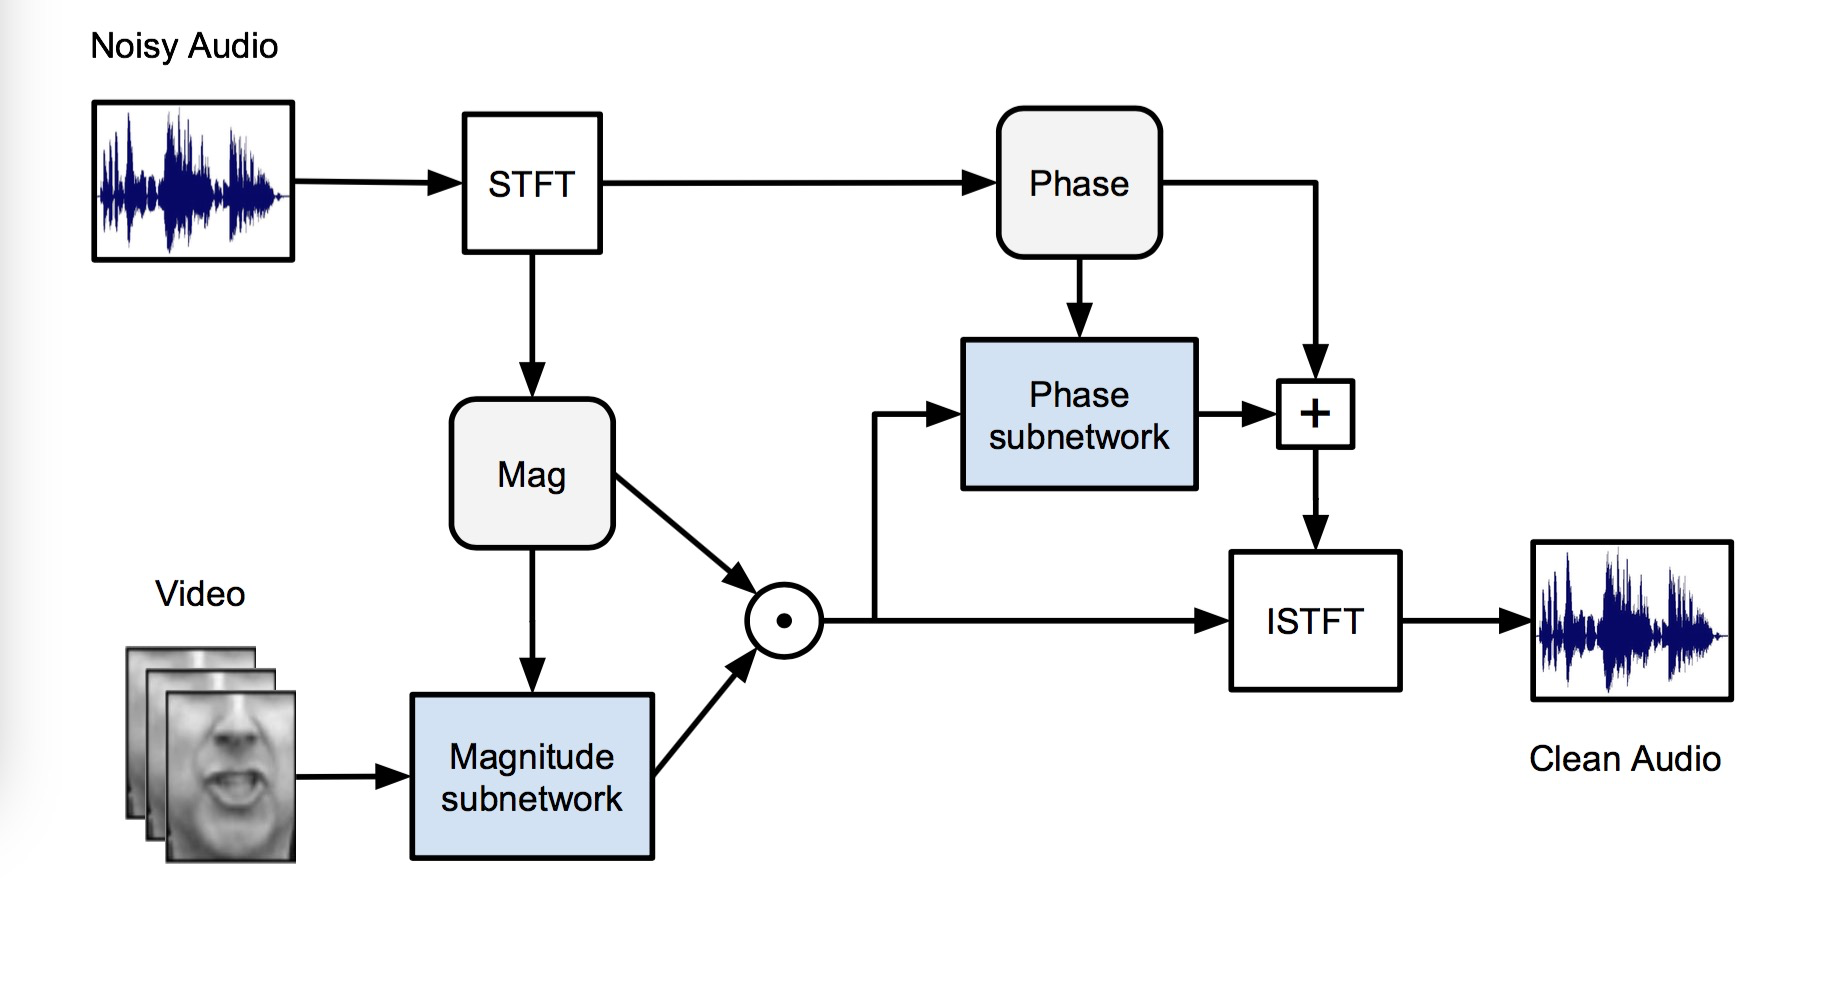
\includegraphics[scale=0.19]{fig3.png}
\caption{Audio-visual speech enhancement architecture}
\label{fig:framework}
\end{figure}

This method requires training of a generalized method of moments (GMM) to model audio and visual speech features, so that the correspondence between the audio and visual features can be used to estimate the audio features from the given videos, since this correspondence has been proposed to be valid by several studies in \cite{5} and \cite{6}.\\

%%% 11-8 12-9 13-10 14-11 15-12 16-13
In 2017, A. Gabbay et, al. \cite{8} Implemented a model that can extract a specific visible speaker’s voice from the similar background noise environments using video data and audio spectrograms. In their study, for unconstrained environments, the separation of the specific speaker requires (i) a sequence of video frames showing the mouth of the speaker; and (ii) a spectrogram of the noisy audio. The source of the audio and video then went through encoder respectively then embedded into fc-layers. Encoding module is composed of a dual tower Convolutional Neural Network in order to make the input from audio/video source have the same embedded representing feature. The video encoder and the audio encoder functions different roles. The video encoder crops from the center of the mouth region of the frames then feed the consecutive gray-scaled cropped frames to consecutive convolution layers (note the layers using Batch Normalization \cite{9} and Leaky-ReLU \cite{10} mathematic matrix processing to filter the frames). The audio encoder receives the input audio spectrogram clips correspond to the video frames fed into the video encoder. The audio encoder also uses convolution layers with Batch Normalization \cite{9} and Leaky-ReLU \cite{10} to filter the audio clips. Both encoders result in the feature vector with the same embedding as output. The two encoders output shared representation to consecutive fully-connected layers. An audio decoder is accepting the data passed through consecutive fully-connected layers with transposed convolution layers to represent the enhanced speech.\\

\begin{figure}[H]
%\centering
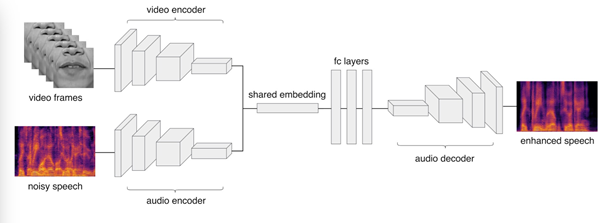
\includegraphics[scale=0.60]{fig4.png}
\caption{Audio/video encoder and decoder model for the study below}
\label{fig:framework}
\end{figure}
 
Aside from the model with video and magnitude of the audio signal example above, \cite{11} in 2017, J.-C. Hou et, al. Introduced a voice enhancement model based on neural network training from a variety of noise features that is able to enhance specific speaker’s voice pattern from different kinds of noise backgrounds. The model incorporates audio and visual streams into a unified network model \cite{12}. Using AVDCNN as the audio-visual encoder-decoder network to perform the voice enhancing job. Where AVDCNN is for Audio-Visual Deep Convolutional Neural Network. Similar to the model introduced by A. Gabbay et al., the model introduced by J.-C. Hou et, al. processes audio and visual streams using two independent convolutional neural networks. A fusion network is following the two convolutional neural networks to fuse them together with maximum pooling layer and fully-connected layer \cite{11}.
This model uses back-propagation to jointly learn the parameters in an end-to-end manner \cite{12}.\\

\begin{figure}[H]
%\centering
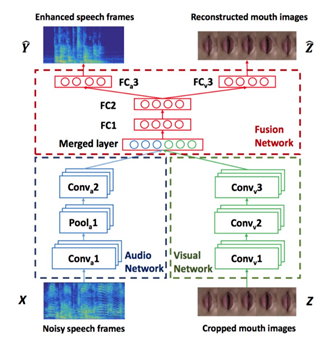
\includegraphics[scale=0.38]{fig5.png}
\caption{Construction of the AVDCNN model for the study above}
\label{fig:framework}
\end{figure}

\section{Data Set}
In order to generate a model for speech recognition and noise removal, we need a large dataset for training and testing the model, one suitable option is VoxCeleb2, which is also used in \cite{7}. It is an open-source media that contains huge amount of audio-visual speaker recognition dataset that we can use in our convolutional neural network training process, which will be discussed in later section. The study proposed in \cite{7} presents a deep CNN based neural speaker embedding system called VGGVox, which is trained to project the voice signal spectrum to Euclidean space, where the Euclidean distance represent the similarity of speakers.\\

\begin{figure}[H]
%\centering
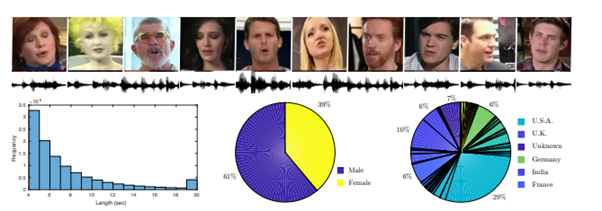
\includegraphics[scale=0.6]{figure3.png}
\caption{Top row: Examples of faces from the VoxCeleb2 dataset.\\Bottom row: (left) distribution of utterance lengths in the dataset – length shorter than 20s are binned in 1s intervals and all utterances of 20s+ are binned together; \\(middle) gender distribution and (right) nationality distribution of speakers. \cite{7}}
\label{fig:framework}
\end{figure}

With each selected audio segment, we transfer the .wav file into image file so that it displays the power spectrogram of the audio. Then we generate noise signals upon this spectrogram to obtain a noisy audio spectrogram that can be later used for training purpose.\\



%%% add words %%%


\section{Proposed Method}
The algorithm requires audio signal with diversity aspect of noise interacted with the original speaker voice.\\
In order to create original speaker voice with different kinds of noise mixure we used pysndfx package \cite{19} to add different kinds of noise to the given '.wav' file. \\
The pysndfx package applies audio effects such as reverb and EQ directly to audio files or NumPy ndarrays. The pysndfx package is a lightweight Python wrapper for SoX - Sound eXchange. Where Sox is a cross-platform command line utility that can convert various formats of computer audio files in to other formats. It can also apply various effects to these sound files, and SoX can play and record audio files on most platforms. \cite{20} The pysndfx supports effects range from EQ and compression to phasers, reverb and pitch shifters. Before importing the pysndfx package the terminal should be installed the package related application. (using pip command to install the package related application)\\

We added mixured level of highshelf, lowshelf filters and reverb, phaser, delay effects to the oriaginal sound and outputed the prcessed sound file and comparsion spectrogram.\\

A low shelf will either cut or boost signals below a c.o.f. in a manner resembling a shelf, or an equal strength amplitude band past the rolloff. A high shelf filter will either cut or boost signals above a c.o.f. similarly.
Where c.o.f stands for cutoff frequency at the point a specific frequency component would have lost approximately half the power (-3 dB) of unaffected frequencies, often referred to as the half-power point. A common synthesis technique is to sweep the cutoff frequency up or down to provide a 'spectral shape' to a sound over time. Cutoff frequencies are usually controlled by an envelope generator or an oscillator (timbre modulation).\cite{21}\\
%HLshelf.jpeg

\begin{figure}[H]
%\centering
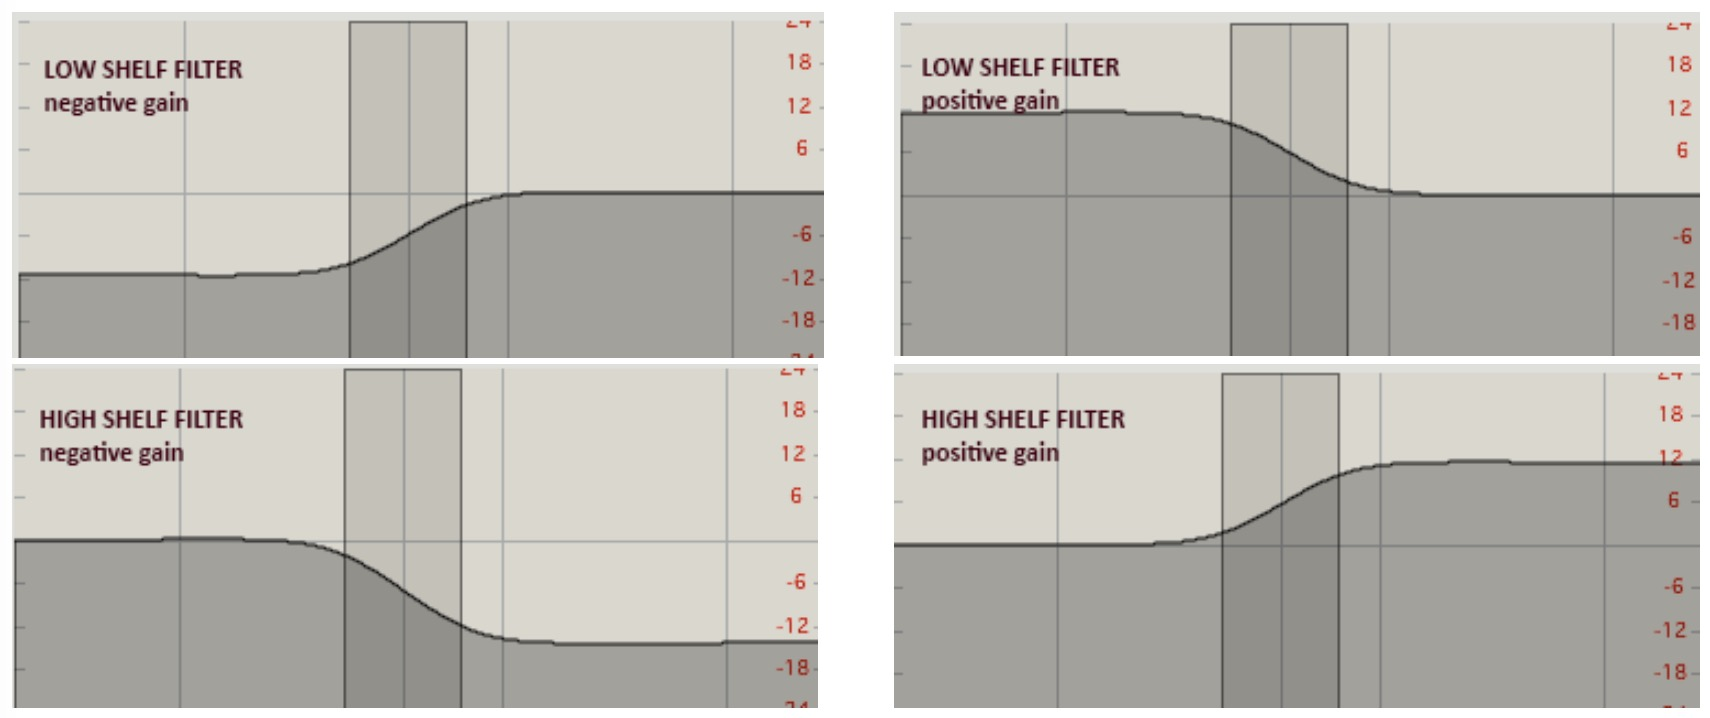
\includegraphics[scale=0.15]{HLshelf.jpeg}
\caption{Shelf transfer function \cite{21}}
\label{fig:framework}
\end{figure}


In detail, The analog transfer function for a low shelf is:\\
%%high_shelf_formula.png%%	\cite{22}
\begin{figure}[H]
%\centering
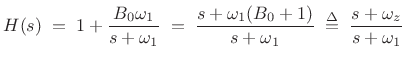
\includegraphics[scale=0.60]{high_shelf_formula.png}
\caption{Low shelf transfer function \cite{22}}
\label{fig:framework}
\end{figure}

where $B_0$ is the dc boost amount (at s = 0), and the high-frequency gain (s = ∞) is constrained to be 1 . The transition frequency dividing low and high frequency regions is w1 . See Appendix E for a development of s-plane analysis of analog (continuous-time) filters. \cite{23}\\
A high shelf is obtained from a low shelf by the conformal mapping (s <-- 1/s) , which interchanges high and low frequencies.\\
%%high_shelf_formula2.png%%  \cite{22}
\begin{figure}[H]
%\centering
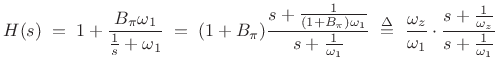
\includegraphics[scale=0.60]{high_shelf_formula2.png}
\caption{High shelf transfer function \cite{22}}
\label{fig:framework}
\end{figure}

In this case, the dc gain is 1 and the high-frequency gain approaches.\\
%%shelf_formula3%%
\begin{figure}[H]
%\centering
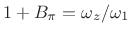
\includegraphics[scale=0.60]{shelf_formula3.png}
%\caption{High shelf transfer function \cite{22}}
\label{fig:framework}
\end{figure}

Low and high shelf filters are typically implemented in series, and are typically used to give a little boost or cut at the extreme low or high end (of the spectrum), respectively. To provide a boost or cut near other frequencies, it is necessary to go to (at least) a second-order section, often called a peaking equalizer. \cite{23}\\

From the below output spectrogram table, low shelf filter tend to lower the wave flux to 0, thus low shelf is able to gain negative to higher wave value and gain positive wave value to a lower value. (Low shelf has a brighter downside while highshelf has a brighter upperside) Vise versa, high shelf is able to gain negative to lower wave value and gain positive wave value to a higher value.\\

\begin{figure}[H]
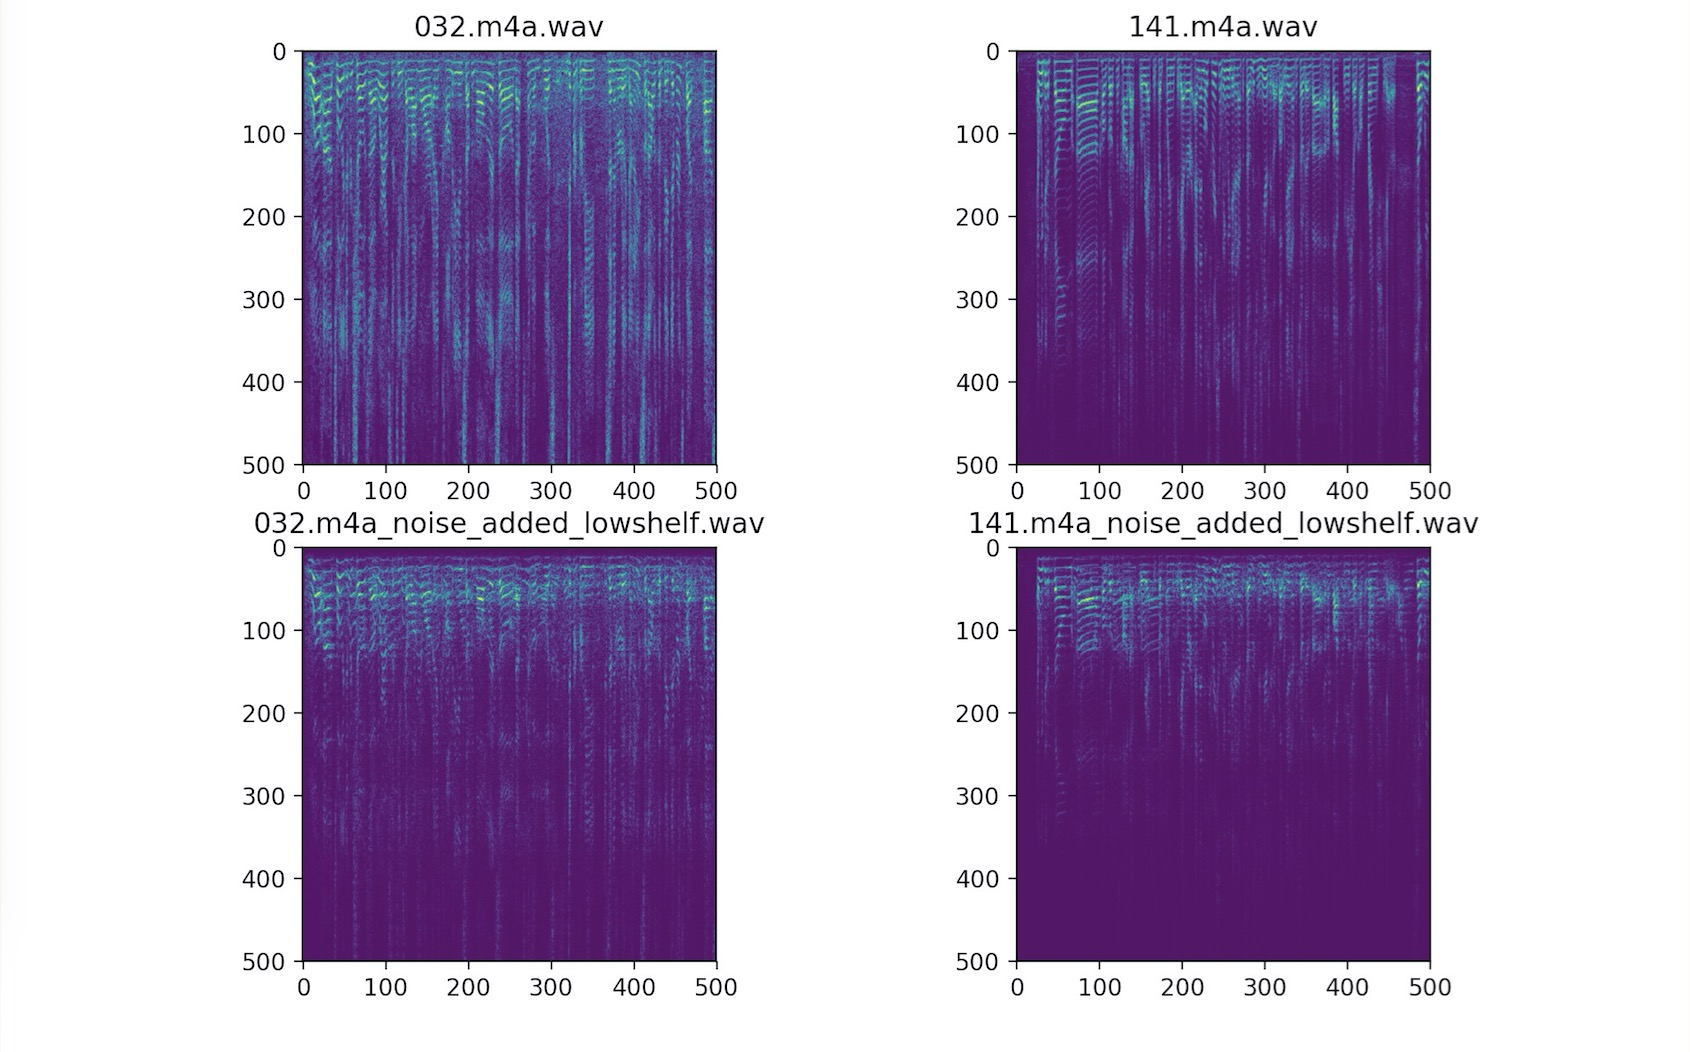
\includegraphics[scale=0.25]{orig_low.jpeg}
\caption{Low shelf}
\label{fig:framework}
\end{figure}

\begin{figure}[H]
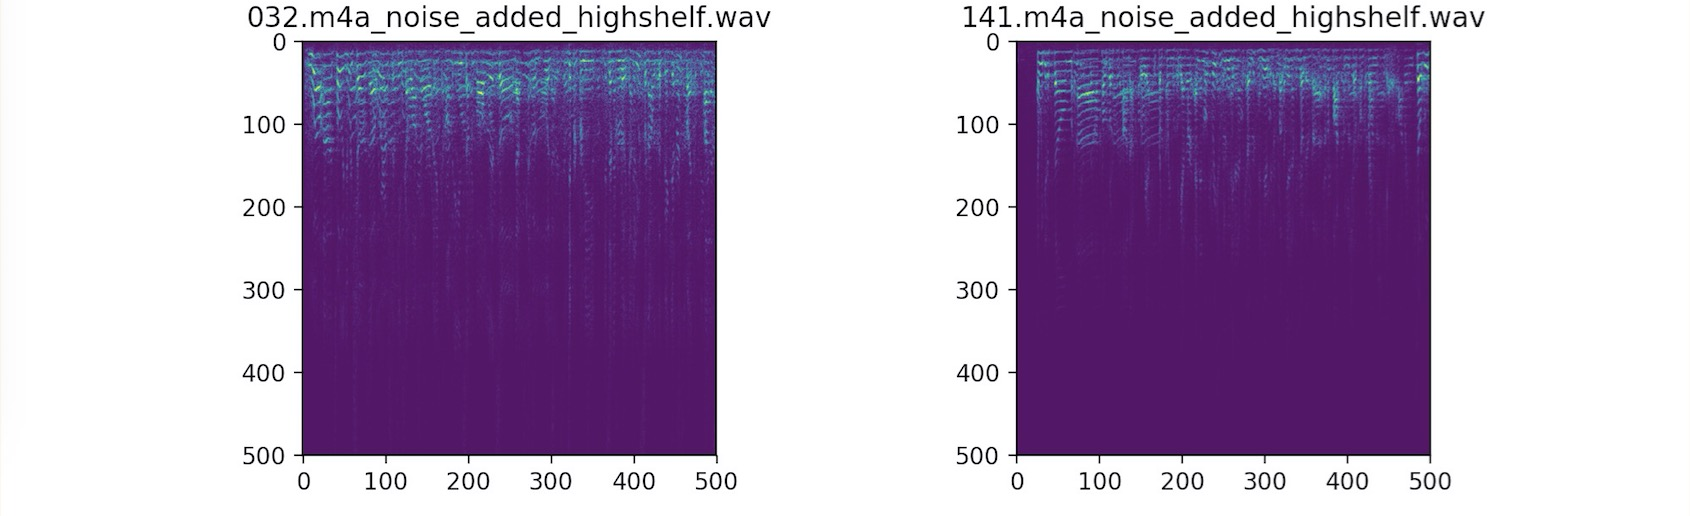
\includegraphics[scale=0.25]{high.jpeg}
\caption{High shelf}
\label{fig:framework}
\end{figure}

\begin{figure}[H]
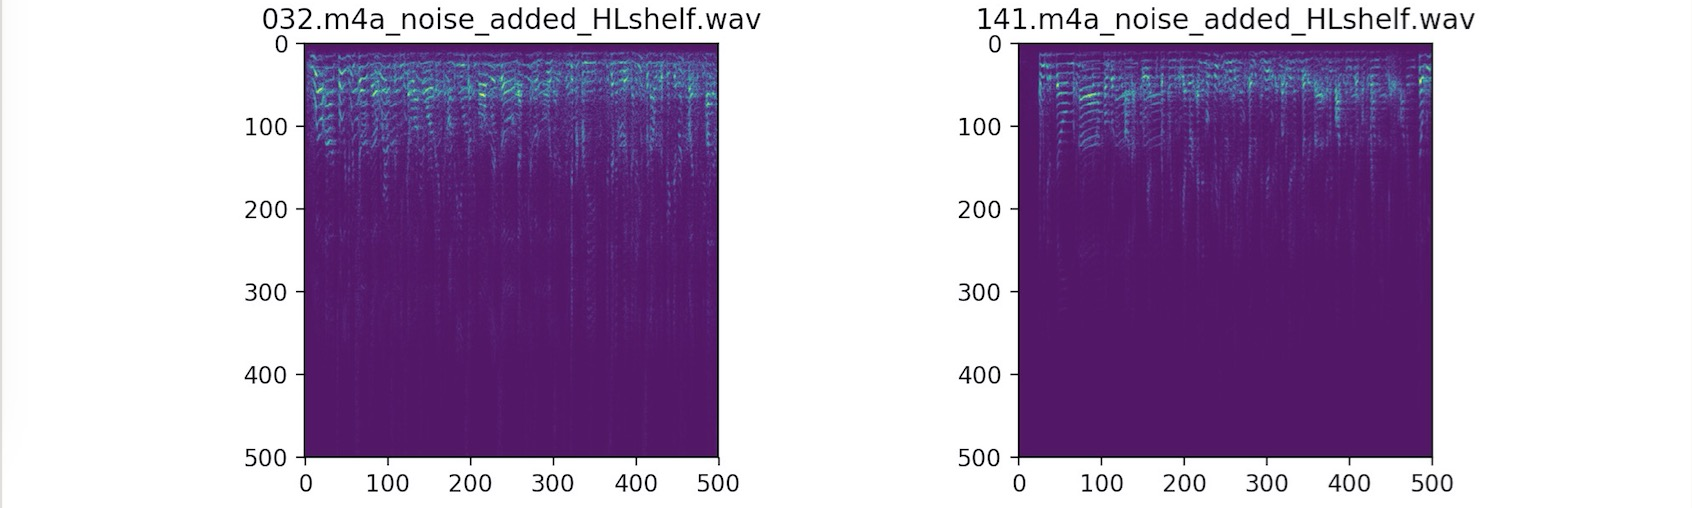
\includegraphics[scale=0.25]{HL.jpeg}
\caption{Low and High shelf (offset each other as comparison to Low shelf and High shelf)}
\label{fig:framework}
\end{figure}



Reverberation is an acoustic phenomenon, in which reflections cause the sound to be prolonged and ring even after the sound source stops \cite{24}

From the below output spectrogram table with Reverberation effect added ......
\begin{figure}[H]
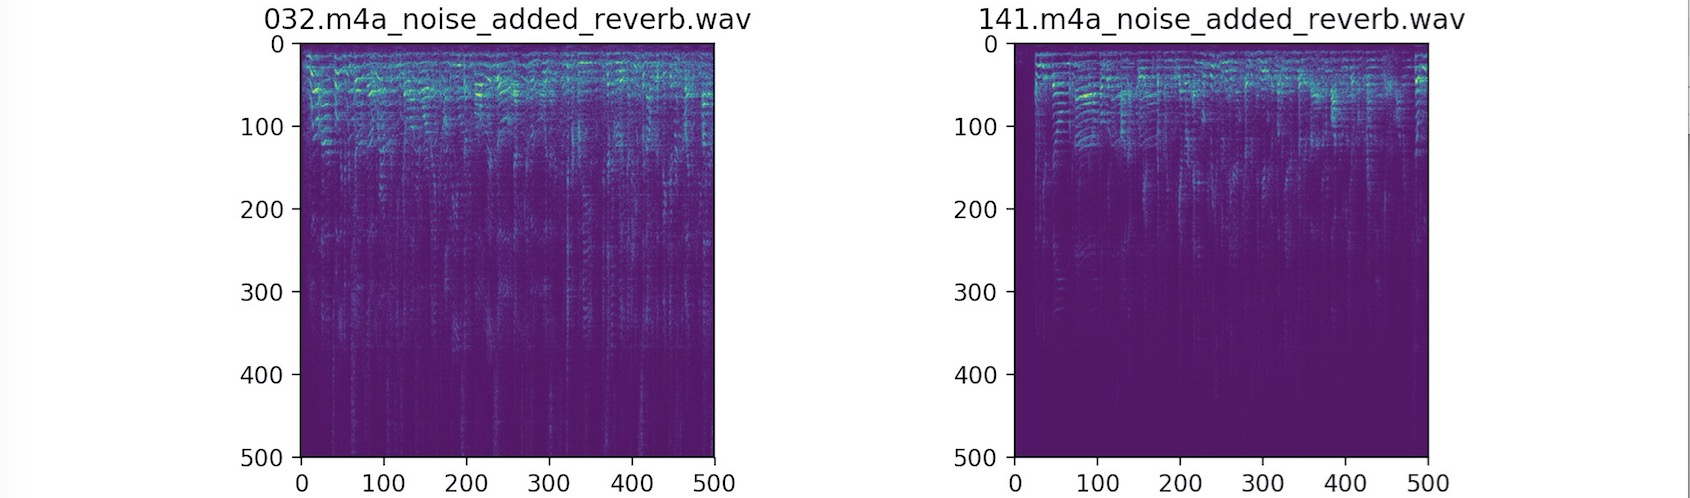
\includegraphics[scale=0.25]{reverb.jpeg}
\caption{Spectrogram with Reverberation effect added to the origainal }
\label{fig:framework}
\end{figure}




\section{Results and Discussion}
Since we are using pre-recorded audio sample, we are not able to control the environment noise in the audio sample, so we add noise signals to the pure spectrogram manually. We test with two forms of noise generation. One using Gaussian method to generate white noise and the other one simply generates random noise. The purpose is to figure out a better approach to mimic white noise in real life and create noisy audio signal close to what we hear in our lives, which would provide better accuracy in testing the model with real noisy speech.\\

We take a sample wav file and transfer it into an image file (figure 12), then using Gaussian noise generation method to create Gaussian noise (figure 13), then add it onto the original spectrogram to create noisy audio spectrogram (figure 14), all three graphs are shown below.\\

\begin{figure}[H]
%\centering
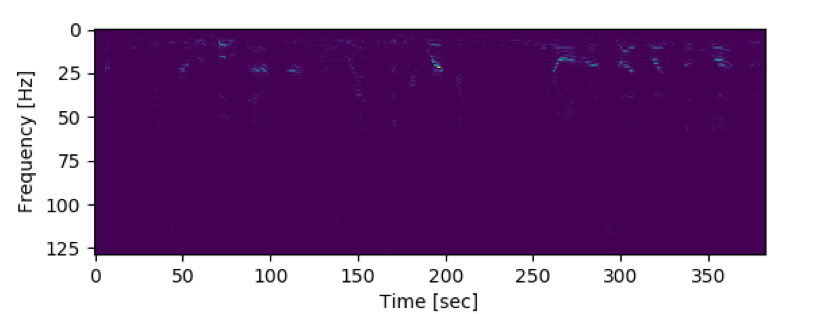
\includegraphics[scale=0.25]{figureA.png}
\caption{Original Spectrogram}
\label{fig:framework}
\end{figure}

\begin{figure}[H]
%\centering
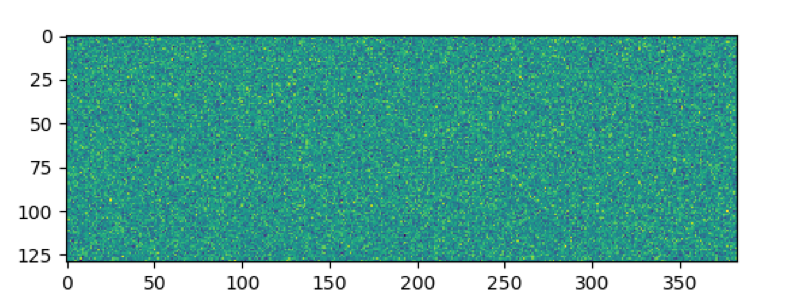
\includegraphics[scale=0.25]{figureB.png}
\caption{Gaussian noise}
\label{fig:framework}
\end{figure}

\begin{figure}[H]
%\centering
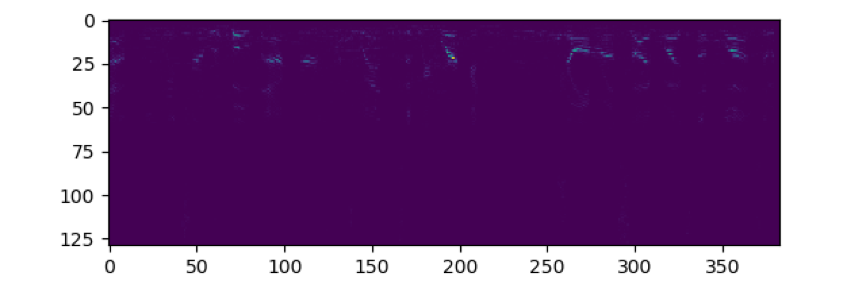
\includegraphics[scale=0.25]{figureC.png}
\caption{Original Spectrogram with Gaussian Noise added}
\label{fig:framework}
\end{figure}

Original Spectrogram with Random Noise added.\\

\begin{figure}[H]
%\centering
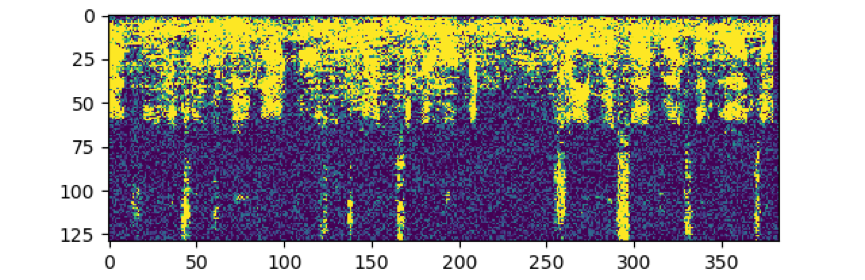
\includegraphics[scale=0.25]{figureE.png}
\caption{Random Noise}
\label{fig:framework}
\end{figure}

\begin{figure}[H]
%\centering
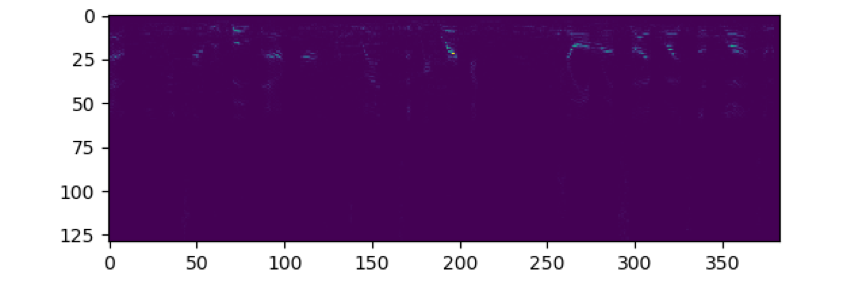
\includegraphics[scale=0.25]{figureD.png}
\caption{Original Spectrogram with Random Noise added}
\label{fig:framework}
\end{figure}

The resulting spectrograms of these two methods appear to be visually similar, yet it is obvious from the noise signal graphs (figure 12 and 15) that they are different. Gaussian method adds noise in a more uniform way which is more common in real life where the white noise permutes into speakers’ audio signals uniformly. The random method fulfills the task in all aspects, but it will not be as effective in our model during training compare to Gaussian noise addition, for the reason that the noise it generates could not mimic real-life white noise, and this will cause our model to be inaccurately trained. Hence, the Gaussian noise is supposed to be a better choice as white noise addition method for white noise addition onto wav file.\\

\section{Conclusion}
We did not fully accomplish the goal we set for this project, so there is not yet a confirmable conclusion about the topic we were discussing about. Since this project is intuited by another published paper\cite{18}, the core concept is determinant. We did reach some partial result of functions required in this project. Gaussian noise generation requires fewer number of operations and achieves a more satisfying result in simulating environmental white noise.

\begin{thebibliography}{4}

\bibitem{1} M. Anusuya and S. K. Katti, “Speech recognition by machine, a review,” arXiv preprint arXiv:1001.2267, 2010.


\bibitem{2} Z.Jinand D.Wang,“A supervised learning approach to monaural segregation of reverberant speech,” IEEE Transactions on Audio, Speech, and Language Processing, 2009.


\bibitem{3}  A. Ephrat, T. Halperin, and S. Peleg, “Improved speech reconstruction from silent video,” in ICCV 2017 Workshop on Computer Vision for Audio-Visual Media, 2017.


\bibitem{4} F.KhanandB.Milner,“Speaker separation using visually-derived binary masks,” in AVSP, 2013


\bibitem{5}  H. Yehia, P. Rubin, and E. Vatikiotis-Bateson, “Quantitative association of vocal tract and facial behavior,” Speech Communication, vol. 26, no. 1, pp. 23–43, Oct. 1998.


\bibitem{6} I. Almajai and B. Milner, “Visually-derived Wiener filters for speech enhancement,” IEEE Trans. Audio, Speech and Language Processing, vol. 19, no. 6, pp. 1642–1651, Aug. 2011.


\bibitem{7} J. S. Chung, A. Nagrani, , and A. Zisserman, “VoxCeleb2: Deep speaker recognition,” arXiv preprint arXiv:1001.2267, 2018.


\bibitem{8} A. Gabbay, A. Shamir, and S. Peleg, “Visual Speech Enhancement using Noise-Invariant Training,” arXiv preprint arXiv:1711.08789, 2017.


\bibitem{9} S. Ioffe and C. Szegedy. Batch normalization: Accelerating deep network training by reducing internal covariate shift. In ICML’ 15, pages 448–456, 2015.


\bibitem{10} A.L.Maas,A.Y.Hannun,andA.Y.Ng.Rectifier nonlinearities improve neural network acoustic models. In ICML’ 13, volume 30, 2013.


\bibitem{11} J.-C. Hou, S.-S. Wang, Y.-H. Lai, Y. Tsao, H.-W. Chang, and H.-M. Wang, “Audio-Visual Speech Enhancement Using Multi- modal Deep Convolutional Neural Networks,” IEEE Transactions on Emerging Topics in Computational Intelligence, 2018.


\bibitem{12} J.-C. Hou, S.-S. Wang, Y.-H. Lai, J.-C. Lin, Y. Tsao, H.-W. Chang, and H.-M. Wang. Audio-visual speech enhancement based on multimodal deep convolutional neural network. arXiv:1703.10893, 2017.
%%% 11-8 12-9 13-10 14-11 15-12

\bibitem{13} Mandelbrot, Benoit B. "A fast fractional Gaussian noise generator." Water Resources Research 7.3 (1971): 543-553.

\bibitem{14} Helf, Brant M., and Peter L. Chu. "Reduction of background noise for speech enhancement." U.S. Patent No. 5,550,924. 27 Aug. 1996.

\bibitem{15} Kok, Chi-Wah. "Speech enhancement by noise masking." U.S. Patent Application No. 10/875,695.

\bibitem{16} Github: https://github.com/zhr1201/CNN-for-single-channel-speech-enhancement

\bibitem{f}  Github: https://github.com/tstafylakis/Lipreading-ResNet

\bibitem{LR} Github: https://github.com/santi-pdp/segan

\bibitem{17} Loizou, Philipos C. Speech enhancement: theory and practice. CRC press, 2007.

\bibitem{18} Afouras, Triantafyllos, Joon Son Chung, and Andrew Zisserman. "The conversation: Deep audio-visual speech enhancement." arXiv preprint arXiv:1804.04121 (2018).

\bibitem{19} PyPI official document-pysndfx 0.3.6: https://pypi.org/project/pysndfx/ 

\bibitem{20} Github: python-audio-effects. https://github.com/carlthome/python-audio-effects/blob/master/README.md

\bibitem{21} Introduction to Computer Music: University of Indiana
http://www.indiana.edu/emusic/etext/synthesis/chapter4_filters.shtml

\bibitem{22} U. Zölzer, Digital Audio Signal Processing, 
New York: John Wiley and Sons, Inc., 1999.

\bibitem{23} J. O. Smith, Introduction to digital filters: with audio applications. W3K Publishing, 2008.

\bibitem{24} V. V ̈alim ̈aki, J. D. Parker, L. Savioja, J. O. Smith, and J. S. Abel, “Fifty years of artificial reverberation,” IEEE Transactions on Audio, Speech, and Language Processing, vol. 20, no. 5, pp. 1421–1448, 2012.


\end{thebibliography}


% \section*{Appendix: Springer-Author Discount}

% LNCS authors are entitled to a 33.3\% discount off all Springer
% publications. Before placing an order, the author should send an email,
% giving full details of his or her Springer publication,
% to \url{orders-HD-individuals@springer.com} to obtain a so-called token. This token is a
% number, which must be entered when placing an order via the Internet, in
% order to obtain the discount.

\end{document}
